\section{Estadísticos Z y t}

\begin{enumerate}
	\item Suponga que el valor del parámetro asumido en la hipótesis nula es $Ao$. 
	\item Tomemos
	una muestra aleatoria de 100 o 1000 personas o eventos del evento. 
	\item Calculemos
	la media del parámetro, por ejemplo la edad promedio de una ciudad, el tiempo medio de suministro de la pizza, la media
	ingresos, etc. 
	\item Podemos llamarlo $A$.
\end{enumerate}




El estadístico $Z$ se calcula para convertir una variable normalmente distribuida (por ejemplo, la distribución de la media poblacional de edad) a una distribución normal estándar.
%  Esto es porque los valores de problemaabilidad para una variable que sigue a la distribución normal estandarizada se puede obtener de una tabla precalculada.


El estadístico $Z$ se da por la siguiente fórmula:
\begin{align}
	\label{zStat}
	Z=\dfrac{A-A_{0}}{{\sigma}/{\sqrt{n}}}
\end{align}
donde $\s$ es la desviación estándar de la población y $n$ es el número de personas en la muestra


Ahora, debemos considerar dos casos

\paragraph{Prueba Z (distribución normal)}
El investigador conoce a desviación estándar del parámetro de su experiencia pasada.



Un buen ejemplo de esto es el caso del tiempo de entrega de una pizza.  En este caso \eqref{zStat} seguirá una distribución normal y los valores normalizados se conocerán como \emph{valores Z}.

\paragraph{Prueba t (distribución t de Student) }
En este caso, el investigador no conoce la desviación estándar de la población.



Esto puede pasar porque:
\begin{itemize}
	\item No existen tales datos en algún registro histórico;
	\item o el número de eventos o personas es demasiado pequeño para suponer una distribución normal.
\end{itemize}


En este caso, la media y la desviación estándar son desconocidas, y la expresión asume una distribución diferente a la normal llamada \emph{distribución $t$ de Student}.



El valor estandarizadas en este caso es llamado \emph{$t-$valor} y la prueba es llamada \emph{prueba-$t$}.


\paragraph{Distribución t de Student}
\begin{quote}
	La distribución de Student fue descrita en 1908 por William Sealy Gosset. Gosset trabajaba en una fábrica de cerveza, Guinness, que prohibía a sus empleados la publicación de artículos científicos debido a una difusión previa de secretos industriales. De ahí que Gosset publicase sus resultados bajo el seudónimo de Student. \footnote{
		\href{https://es.wikipedia.org/wiki/Distribuci\%C3\%B3n\_t\_de\_Student\#Historia}{Wikipedia: Distribución $t$ de Student}
	}
\end{quote}


\begin{figure}
	\centering
	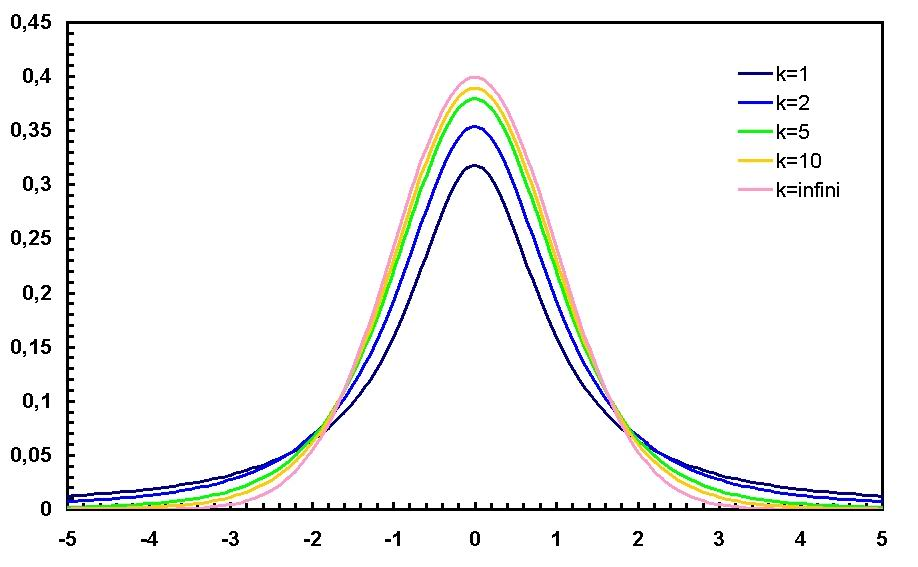
\includegraphics[height=5cm,keepaspectratio=true]{./images/Student_densite_best.jpg}
	% Student_densite_best.jpg: 0x0 pixel, 300dpi, 0.00x0.00 cm, bb=
	\caption{De The original uploader was Thorin de Wikipedia en francés - Transferido desde fr.wikipedia a Commons., CC BY-SA 1.0, https://commons.wikimedia.org/w/index.php?curid=1878902}
	\label{fig:tPDF}
\end{figure}




\begin{figure}
	\centering
	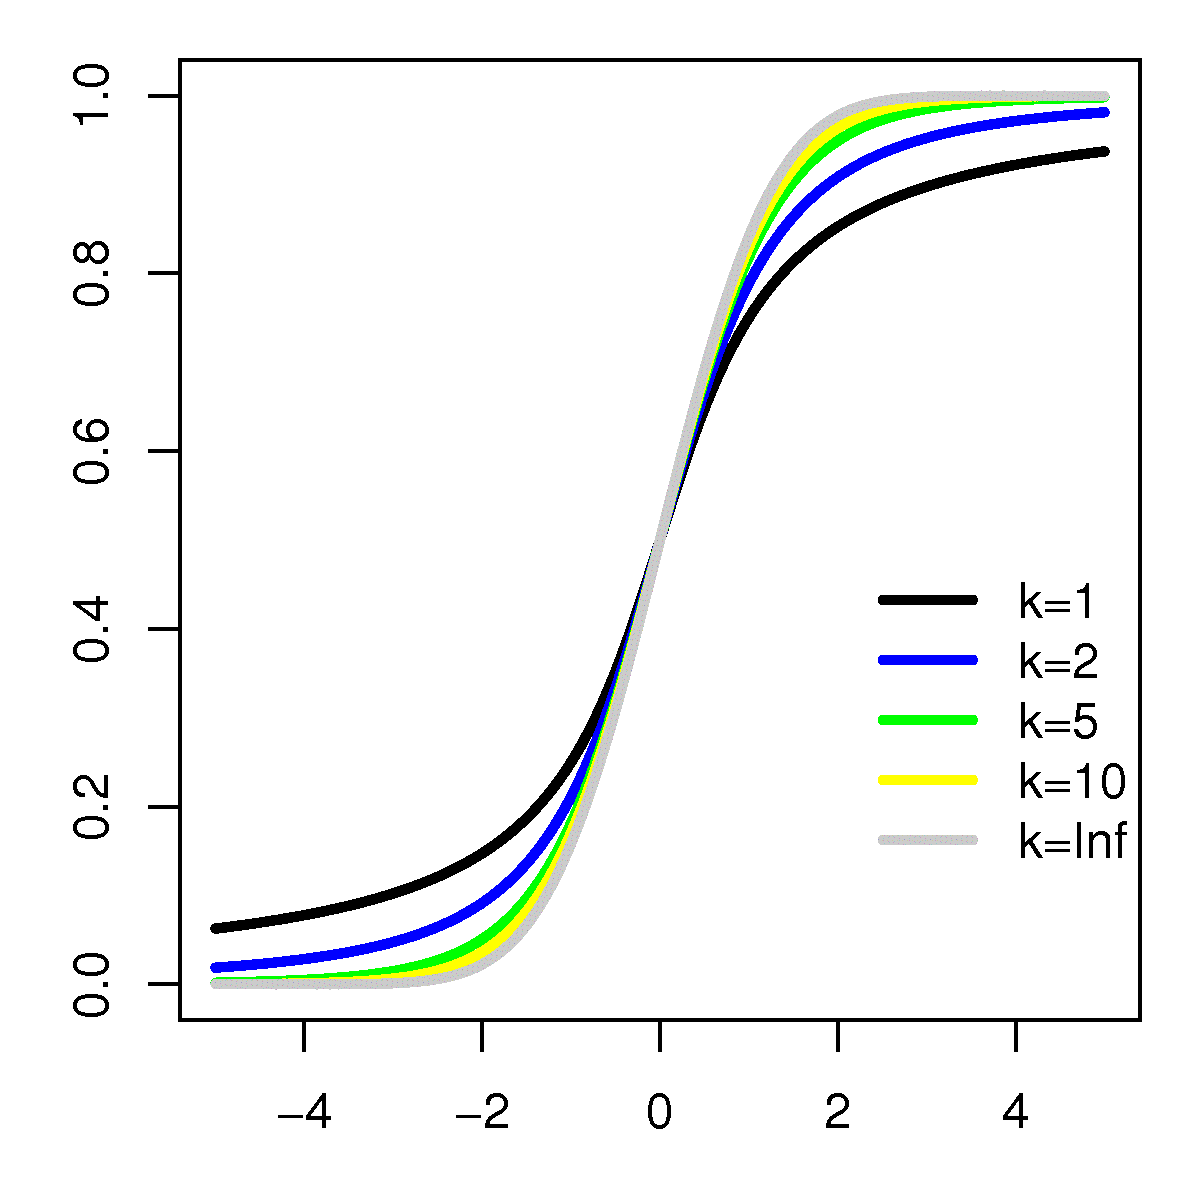
\includegraphics[height=5cm,keepaspectratio=true]{./images/T_distributionCDF.png}
	% T_distributionCDF.png: 0x0 pixel, 300dpi, 0.00x0.00 cm, bb=
	\caption{De Desconocido, CC BY-SA 3.0, https://commons.wikimedia.org/w/index.php?curid=788691}
	\label{fig:tCDF}
\end{figure}

\begin{lstlisting}[language=Python, caption=Distribución $t$ en \texttt{Python}]
	from scipy import stats
	import numpy as np
	import matplotlib.pyplot as plt
	
	def ft(x, nu):
	return stats.t.pdf(x, df=nu)
	def Ft(x, nu):
	return stats.t.cdf(x, df=nu)
	x = np.arange(-4,4,0.01)
	yd = ft(x,30)
	yc = Ft(x,30)
	
	fig, ax = plt.subplots()
	plt.plot(x, yd, 'r', linewidth=2)
	plt.plot(x, yc, 'b', linewidth=2)
	plt.ylim(ymin=0)
	plt.show()
\end{lstlisting}



\begin{figure}
	\centering
	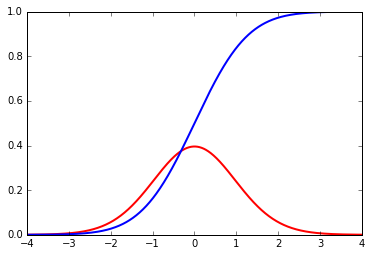
\includegraphics[height=7cm,keepaspectratio=true]{./images/tCDF.png}
	% tPDF.png: 0x0 pixel, 300dpi, 0.00x0.00 cm, bb=
\end{figure}



El parámetro \texttt{df} se le conoce como \emph{grados de libertad} y generalmente se denota como $\nu$ (la letra \texttt{nu} griega).


Si una variable aleatoria $X$ tiene distribución $t$ con $\nu$ grados de libertad, entonces
\begin{align}
	\mu_{X}=0, \; \s^{2}_{X}=\dfrac{\nu}{\nu-2}
\end{align}



\begin{ejemplo}
	Consideremos una variable con distribución $t$ y $\nu=9$ grados de libertad. Encuentre el valor de $t$ para el cuál el área a la derecha sea $0.05$ pero el total del área sin sombrear sea $0.90$.
	\begin{figure}
		\centering
		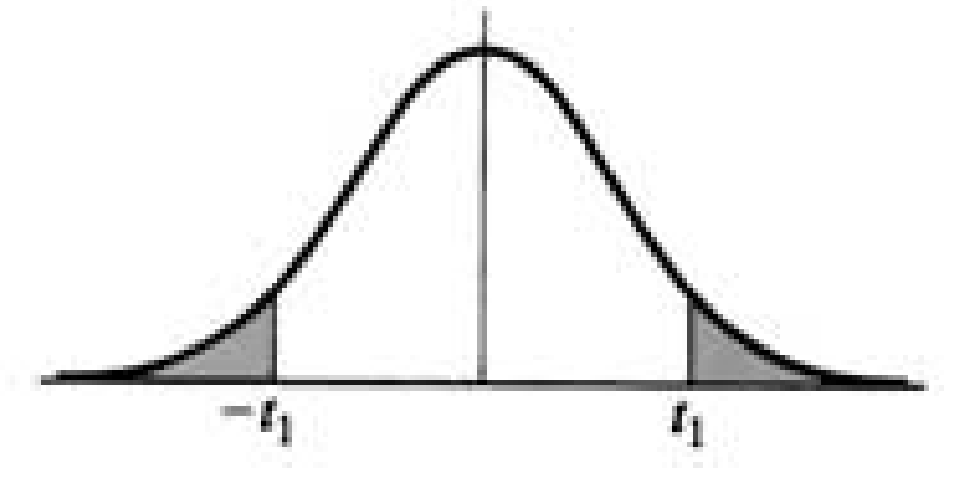
\includegraphics[height=3cm,,keepaspectratio=true]{./images/tExample.png}
		% tExample.png: 0x0 pixel, 300dpi, 0.00x0.00 cm, bb=
	\end{figure}
	
\end{ejemplo}


[]{tExample.py}
\begin{lstlisting}[language=Python]
	from scipy import stats
	import numpy as np
	import matplotlib.pyplot as plt
	
	def tp(x, nu):
	return stats.t.ppf(x, df=nu)
	
	print tp(0.05, 9)
	##-1.83311293265
	print tp(1-0.05, 9)
	##1.83311293265
\end{lstlisting}

\paragraph{Varianza muestral}
\begin{align}
	S^{2}=\sum\dfrac{\left( A_{i}-A_{0} \right)^{2}}{n-1}
\end{align}


\paragraph{Estadístico t}
\begin{align}
	t = \dfrac{\left( A-A_{0} \right)}{S/\sqrt{n}}
\end{align}


